\subsection{Fault Trees, Forests, and Minimal Cut Sets}
\label{sec:saArtifacts}
%\danielle{Move this paragraph to where it makes sense.} Safety analysis has traditionally been performed manually, but with the rise of model checking and the improvement of its capabilities, the world of safety analysis began to see its powerful benefits~\cite{hinchey2012industrial, liggesmeyer1998improving, coudert1993fault, Bozzano:2010:DSA:1951720,bozzano2003esacs}. There arose multiple ways of viewing the system and fault models, various ways of automating the capture of safety pertinent information, and a number of tools that addressed various issues that arose. In this section, we discuss the state of the practice and how formal methods has been applied in the domain of safety assessment research.

A \emph{fault tree} is a directed acyclic graph whose leaves model component failures and whose gates model failure propagation. The system failure under examination is the root of the tree and is called the \emph{top level event}. The \emph{basic events} are the events that can occur in the system which lead to the top level event and in the graphical model, these correspond to the leaves. A {\em fault forest} is simply a set of fault trees. The gates in the fault tree describe how failures propagate through the system. Each gate has one output and one or more inputs. For example in Figure~\ref{fig:introFT}, the AND gate on the bottom left has two inputs and one output. The leaves of the tree represent the basic events of the system and in the case of this fault tree, these four basic events can be found in the \textit{minimum cut sets} for this top level event. A minimal cut set is the minimal set of basic events that must occur together in order to cause the top level event to occur. Finding these sets is important to fault tree analysis and has been an active area of interest in the research community since fault trees were first described in Bell Labs in 1961~\cite{historyFTA, 0f356f05e72f43018211b36f97c8854a}. 

\begin{figure}[h]
\begin{center}
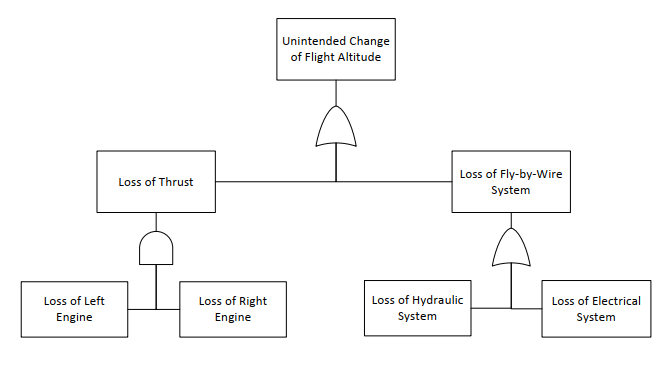
\includegraphics[width=8cm]{images/ft.png}
\caption{A Simple Fault Tree} \label{fig:introFT}
\end{center}
\end{figure}

Figure~\ref{fig:introFT} shows a simple example of a fault tree. In this example, the top level event corresponds to an aircraft having an unintended change of altitude. In order for this event to occur, there must be either a loss of thrust or the loss of a Fly-by-Wire system. This is seen through the use of the OR gate below the top level event. The malfunction of both the left and right engines will cause the loss of thrust to occur and the Fly-by-Wire system can be lost if either the hydraulic system or the electrical system were to malfunction. The MCSs for this example are \{Loss of Left Engine, Loss of Right Engine\}, \{Loss of Hydraulic System\}, and \{Loss of Electrical System\}. 

%There are two main types of FTA that we differentiate here as \textit{qualitative} analysis and \textit{quantitative} analysis. In qualitative analysis, the structure of the fault tree is considered and the cut sets are a way to indicate which combinations of component failures will cause the system to fail. On the other hand, in quantitative analysis the probability of the TLE is calculated given the probability of occurance of the basic events. 

\textbf{History of Fault Trees} 
Since the early days of safety engineering, fault tree analysis has been a primary method of determining safety of a system and showing the behavior of the system (with respect to its requirements) in the presence of faults~\cite{0f356f05e72f43018211b36f97c8854a,vesely1981fault}. Fault tree analysis requires one to explore the faults of the system and their effects on system behavior to determine minimal fault configurations that may violate requirements. From the beginning of fault tree analysis in the 1960s, algorithms worked directly with the fault tree structure to produce minimal cut sets~\cite{10020219108,semanderes1971elraft}. In essence, these algorithms represented each AND/OR gate as a boolean expression and then performed simplification to relate the basic events to the top level event without any gates~\cite{0f356f05e72f43018211b36f97c8854a}. In 1993, Rauzy et al. developed a new approach that converted the fault tree structure into a binary decision diagram (BDD)~\cite{rauzy1993new}. This was a natural way to reduce the Boolean formula into something far more computationally efficient and reducible to even simpler forms. BDDs are still commonly used to perform quantitative and qualitative fault tree analysis~\cite{sinnamon1997new,bryant1986graph,aralia1996computation,reay2002fault,rauzy2007assessment,ge2015quantitative,jiang2018algebraic,banov2019new}.  Other forms of fault tree analysis include Monte Carlo methods~\cite{vesely1970prep}, Markov chains~\cite{boudali2007dynamic}, and variations on BDDs~\cite{minato2001zero}. 




\begin{comment}
\subsubsection{Failure Mode and Effects Analysis}
\danielle{Is this section necessary? If I don't talk about FMEA tables again, cut this.} Failure Mode and Effects Analysis (FMEA) was one of the first systematic ways of performing dependability analysis and is used throughout the safety critical industries~\cite{rausand2003system,Bozzano:2011:SDP:1992983.1992988}. FMEA provides a structured way to list possible failures and their consequences systemwide. If probabilities of failures are known, quantitative analysis can be performed to estimate system reliability and to assign critical significance to potential failure modes or system components~\cite{MilStandardFMEA}. Performing FMEA is often the first step in the fault tree construction, for it shows possible component failures and hence basic events~\cite{0f356f05e72f43018211b36f97c8854a}. Typically, the failure modes of the components at a given level are considered; the objective it to identify the effects of the failure modes at that level - and usually higher levels - of the design. The FMEA results are often presented in tabular form (FMEA Table). FMEA tables vary in form, but almost always include failure mode definitions, the operational mode in which the failure can occur, and possible causes of the failure~\cite{Bozzano:2010:DSA:1951720}.
\end{comment}
